\documentclass[12pt,a4paper]{article}
\usepackage[czech]{babel}
\usepackage[T1]{fontenc}
\usepackage[utf8]{inputenc}
\usepackage{lmodern}
\usepackage{graphicx}
\usepackage{listings}
\usepackage{url}
% \usepackage{hyperref}
\usepackage{xcolor}
\usepackage{geometry}
\usepackage{dirtree}
\usepackage{lmodern}        % Better font
\usepackage{titling}        % For custom title layout
\usepackage{svg}
\usepackage{float}          % [H] option for figures 
\usepackage{comment}        % For block comments

\graphicspath{ {./img/} }

%===== Hyperlinky =====
\usepackage[colorlinks]{hyperref}
\hypersetup{citebordercolor=1 0 0,
			colorlinks=true,
            % refcolor=red,
			citecolor=red,
			urlcolor=blue,
            linkcolor=black,    % Zde změnit barvu tableofcontents
}

%===== Citace =====
%backend=biber, , sortlocale=cs_CZ,autolang=other, language=czech
\usepackage[style=iso-numeric, backend=biber]{biblatex}
\addbibresource{bibliography.bib}
\DeclareFieldFormat{labelnumberwidth}{\mkbibbrackets{#1}}
\usepackage{csquotes}

\usepackage[most]{tcolorbox}
\tcbset{
  myhighlight/.style={
    colback=gray!10,      % background color
    colframe=gray!85!gray, % border color
    boxrule=0.8pt,          % border thickness
    arc=4pt,                % rounded corners
    left=6pt, right=6pt, top=6pt, bottom=6pt, % padding
    fonttitle=\bfseries
    % title=Important
  }
}

\geometry{a4paper, margin=2.5cm}

\lstset{
    basicstyle=\small\ttfamily,
    keywordstyle=\color{blue},
    commentstyle=\color{green!50!black},
    stringstyle=\color{red},
    numbers=left,
    numberstyle=\tiny\color{gray},
    stepnumber=1,
    numbersep=5pt,
    backgroundcolor=\color{white},
    showspaces=false,
    showstringspaces=false,
    showtabs=false,
    frame=single,
    tabsize=4,
    captionpos=b,
    breaklines=true,
    breakatwhitespace=false,
    framexleftmargin=0mm,
    framexrightmargin=0mm,
    framesep=2mm,
    xleftmargin=5mm,
    xrightmargin=0mm,
    language=Python
}

\setlength{\parindent}{0pt}    % No indentation
\setlength{\parskip}{1em}

% Formátování titulku
% \pretitle{%
%   \begin{center}
%     
\includegraphics[width=0.6\textwidth]{img/FIT_color_CMYK_EN.eps}\\[\bigskipamount]
%     \Huge\bfseries
% }
\pretitle{\begin{center}\Huge\bfseries}
\posttitle{\par\end{center}\vskip 0.5em}
\preauthor{\begin{center}\Large}
\postauthor{\end{center}}
\predate{\begin{center}\small}
\postdate{\end{center}}

\title{KNN: Rozpoznání matematických rovnic}
\author{Jakub Málek\\Tomáš Milostný\\Marek Večeřa}
\date{\today}

\begin{document}

\maketitle
\thispagestyle{empty}   % První stránka bez číslování

\begin{center}
    \large \texttt{\{xmalek17,xmilos02,xvecer31\}@vutbr.fit.cz}\\[1ex]
    \normalsize Akademický rok 2024/2025
\end{center}

\vspace{10cm}
% ===== LOGO =====
\begin{figure}[H]
    \centering
    
\includegraphics[width=0.6\textwidth]{img/FIT_color_CMYK_EN.eps}
\end{figure}


\newpage
\tableofcontents

\newpage
\section{Úvod}
Tento dokument popisuje problematiku a řešení rozpoznání matematických rovnic. Jedná se o velmi aktuální téma, které se v posledních letech stalo předmětem mnoha výzkumů a aplikací. Rozpoznávání matematických vzorců je důležité pro automatizaci různých úloh, jako je převod tištěných nebo ručně psaných vzorců do digitálního formátu, což usnadňuje jejich zpracování a analýzu.

Zdrojový kód je otevřeně dostupný na \href{https://github.com/malekjakub69/knn-math}{https://github.com/malekjakub69/knn-math}.

\section{Popis úlohy}
Úkolem projektu je vytvoření a natrénování modelu pomocí strojového učení, který bude schopný rozpoznat obrázky matematických výrazů na vstupu a převést je do strojového zápisu. Formát vstupních obrázků jsme si zvolili jako obrázky ručně psaných rovnic, které budou následně převedeny do formátu \LaTeX -- \textbf{offline recognition}.


\section{Přehled existujících řešení}
V celé historii problematiky rozpoznávání ručně psaných matematických rovnic se objevily tři odlišné přístupy~\ref{img:method_history}. Na počátku se jednalo o jednodušší více přímočaré metody označované jako sekvenční řešení~\cite{ukr_survey}.

% ===== Method histoty img =====
\begin{figure}[H]
    \centering
    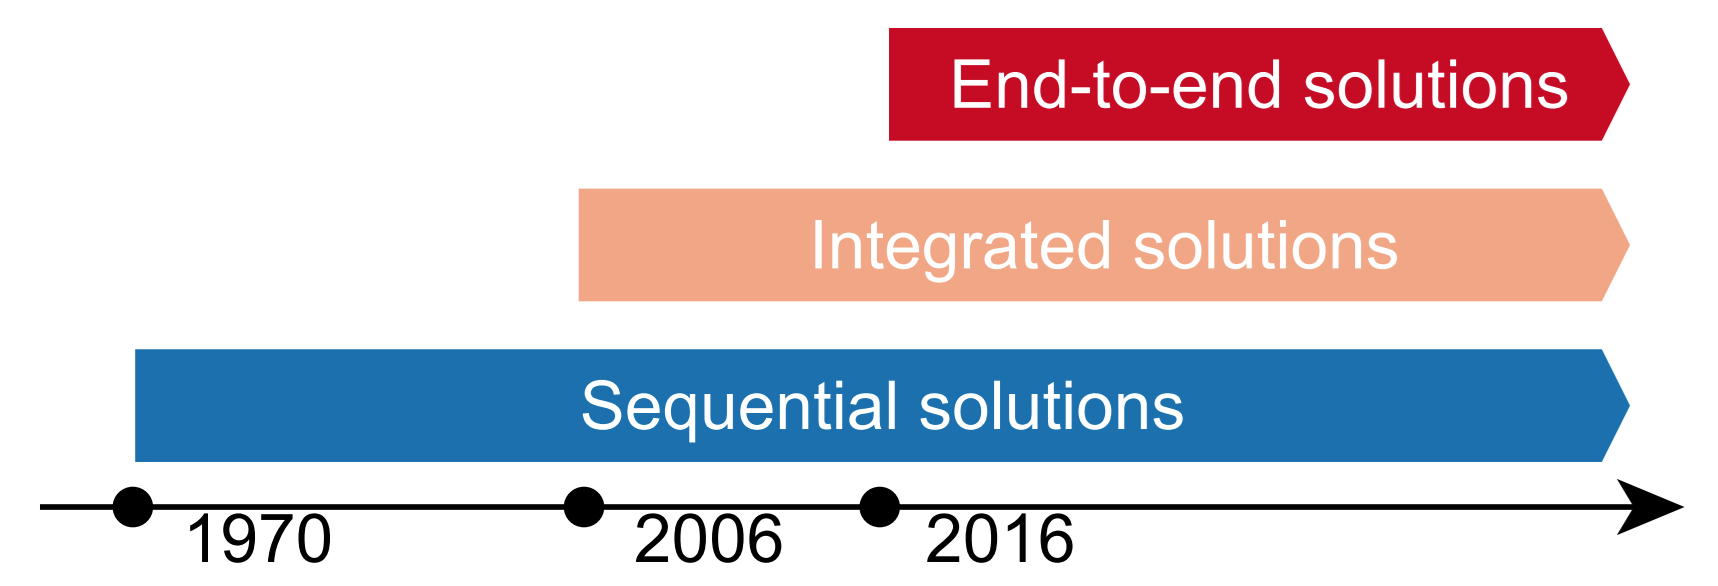
\includegraphics[width=0.6\textwidth]{img/method_history.png}
    \caption{Časový vývoj různých metod pro rozpoznávání matematických vzorců}
    \label{img:method_history}
\end{figure}

\subsection{Sekvenční metody}
Používají princip dekompozice a tuto metodu lze rozložit do několika částí (obrázek~\ref{img:seq_sol}). Modely pracující na tomto principu nejprve (1) rozpoznají jednotlivé symboly a následně provedou (2) strukturní analýzu, kde jednotlivé symboly poskládají do celého výrazu. Rozpoznávání symbolů lze pak dále rozložit na segmentaci jednotlivých symbolů a jejich klasifikaci. Tato metoda o několika krocích má ale nevýhodu v akumulaci chyb během výpočtu jednotlivých kroků.

% ===== Seq. Sol. img =====
\begin{figure}[H]
    \centering
    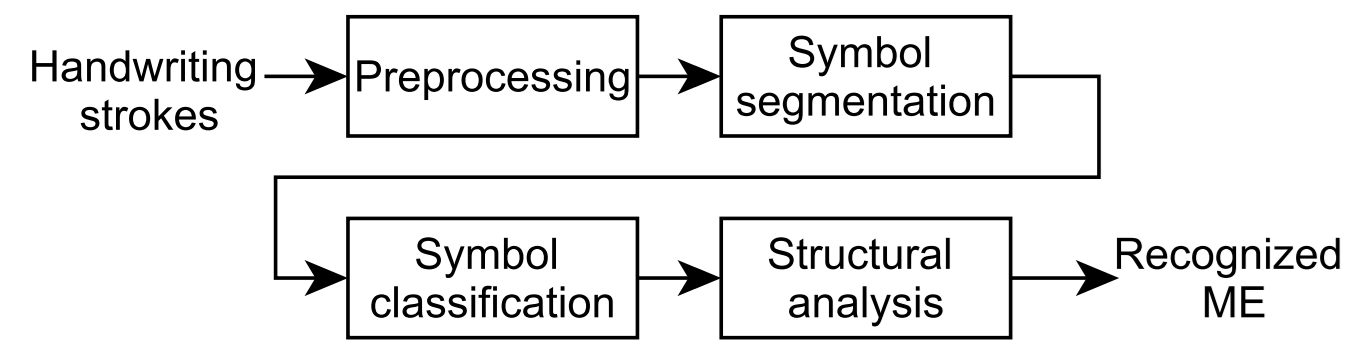
\includegraphics[width=0.6\textwidth]{img/sequential_sol.png}
    \caption{Diagram postupu sekvenčního řešení}
    \label{img:seq_sol}
\end{figure}

\subsection{Integrované metody}
Generují množinu symbolických hypotéz a následně pomocí strukturní analýzy vyberou tu nejlepší na základě znalosti odpovídající gramatiky a sémantiky. Tento přístup je složitější a vyžaduje více výpočetních prostředků, ale může poskytnout lepší výsledky v případě složitějších vzorců.

\subsection{End-to-end metody}
Zatímco předchozí dvě metody řešení problematiky rozpoznávání matematických rovnic byly v posledních dekádách studovány důkladně, \textbf{end-to-end řešení} na principu \textbf{encoder--decoder} se začaly objevovat relativně nedávno. Tento přístup se snaží vyřešit problém rozpoznávání vzorců jako celek, bez rozdělení na jednotlivé části. Používá hluboké učení a neuronové sítě bez jakékoli znalosti konkrétní domény pro tvorbu modelu -- \textbf{data-driven} přístup. Enkodér převede vstup na latentní reprezentaci a dekodér extrahuje skrytou reprezentaci za pomoci attention mechanismu a generuje výstupní sekvenci. 

Jeden z prvních návrhů konkrétní architektury se skládal z \textbf{VGG} sítě, která sloužila jako enkodér \cite{ZHANG_1}. Model dále využíval \textbf{GRU} jako dekodér. Takto navržený systém disponuje přesností okolo 45~\% na datasetech \textbf{CROHME} (Competition on Recognition of Handwritten Mathematical Expressions (HME)), které jsou standardem evaluace modelů pro rozpoznávání matematických vzorců. 

\begin{tcolorbox}[myhighlight]
Evaluační metrika \textbf{expression recognition rate/accuracy} -- vyhodnocuje správnost modelu jak z pohledu jednotlivých symbolů, tak i celkové struktury. Jako správný se výstup považuje v případě, že celkový počet chyb v jednom výstupu není více než 3. 
\end{tcolorbox}

Vylepšení původního návrhu architektury dále zahrnovala nahrazení VGG sítě a použití DenseNet (densely connected conv. network) jako enkodéru \cite{ZHANG_2}. Ve článku \cite{LeAnhDuc} představují end-to-end řešení: kaskáda CNN - feature extractor, BLSTM - encoder a LSTM s attention mechanismem jako dekodér.

V posledním ročníku soutěže CROHME 2023 se objevilo několik návrhů. Vítězný tým představil model skládající se z vrstev CNN a BLSTM pro enkodér a dekodér v podobě attention mechanismu (expression recognition rate 86.95~\%).

Další účastníci se řešení používá DenseNet jako enkodér a 2 různé řešení dekodéru: bidirectional tree decoder a klasický dekodér. S tímto přístupem vznikají 2 modely, jejichž spojením vzniká hybridní model (expression recognition rate 86.95~\%). 

Poslední model představený v soutěži, který uvedeme v této kapitole, je složen ze 2 částí: obrazový model -- CRNN architektura trénovaná na CTC loss funkci, a jazykový model -- LSTM architektura trénovaná pro predikci dalšího \LaTeX~tokenu (expression recognition rate 75.55~\%).

Týmy mají pro tvorbu řešení k dispozici online i offline datasety, které důmyslně používají spolu s augmentací a generováním offline dat z online datasetu pro zlepšení výsledků.


\cite{CROHME_2023}



\section{Popis vlastního řešení}

Na základě provedené rešerše existujících řešení jsme sestavili vlastní NN model založený na \textbf{Vision~Transformer} (ViT) enkodér-dekodér architektuře (poprvé představena v roce 2019) spolu s VGG sítí na vstupu pro prvotní extrakci rysů z obrázku. 


\subsection{Vstupní data}
Použili jsme \href{https://ai.100tal.com/icdar}{oficiální dataset} soutěže ICDAR CROHME 2023 s celkem 30~000 obrázky ručně psaných matematických rovnic (HME) spolu s přiloženými \LaTeX~sekvencemi, které jsme přímo použili jako ground truth.

Dále jsme zkusili trénovací sadu expandovat pomocí generování obrázků HME z offline dat, které jsou k dispozici v mnohem větším množství. K tomuto účelu jsme využili největší dostupný dataset HME -- \href{https://arxiv.org/html/2404.10690v1}{MathWriting}, který obsahuje 230~000 ručně psaných a 400~000 syntetických offline záznamů ve formátu InkML, který ke každému záznamu rovněž obsahoval \LaTeX~ground truth. Pomocí souřadnic jednotlivých tahů offline záznamů jsme byli schopni vykreslit obrazovou reprezentaci a takto celkovou trénovací sadu mnohonásobně rozšířit.

\subsubsection{Augmentace}

Pro zlepšení robustnosti modelu jsme do procesu trénování přidali řadu transformací vstupního obrázku. Konkrétně se aplikují mírné změny výšky a šířky obrázku, změna barev (color jitter), rozmazání dle Gaussova rozdělení, rotace, posuny a přidání náhodného šumu.


\subsection{Model}

Původní baseline řešení představené v rámci checkpointu a videa obsahovalo řadu problémů, které jsme se pokusili vyřešit konzultací a nalezením dalších dříve zmíněných existujících řešení. Aktuální verze modelu \LaTeX~OCR převádí vstupní obrázek na sekvenci tokenů reprezentující \LaTeX~kód s využitím hybridní architektury založené na transformerovém kodéru a dekodéru s přidanými konvolučními vrstvami VGG, patch embeddingem a pozičním kódováním.

\begin{figure}[h!]
    \centering
    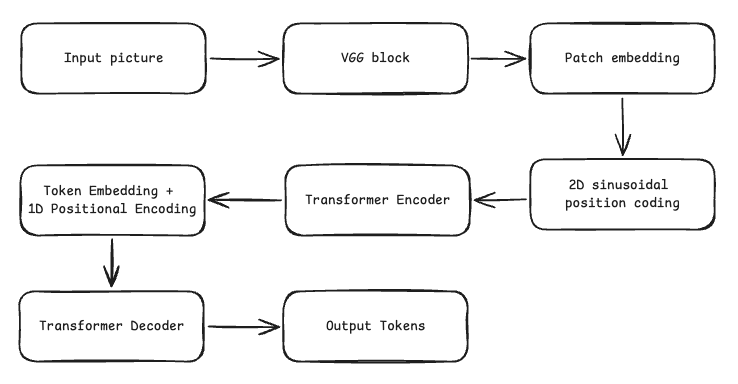
\includegraphics[width=0.75\textwidth]{img/model.png}
    \caption{Architektura modelu \LaTeX~OCR}
    \label{img:seq_sol}
\end{figure}

\subsubsection{Komponenty arhitektury}

\begin{itemize}
    \item \textbf{Vstupní obrázek} - pro zachování správného rozměru se vstupní obrázek nejprve pomocí interpolace změní na pevnou výšku 80 pixelů, přičemž je zachován původní poměr stran, a následně se doplňuje padding tak, aby šířka byla dělitelná velikostí patche.
    \item \textbf{VGG blok} - slouží jako první stupeň extrakce vizuálních příznaků ze vstupního obrázku. Inspirovaný architekturou VGG sítě, používá sekvenci konvolučních vrstev následovaných batch normalizací a ReLU aktivací. Tento blok redukuje prostorové rozměry na polovinu (tedy výšku 40 pixelů) pomocí MaxPoolingu a současně zvyšuje počet kanálů na 64, čímž vytváří bohatší reprezentaci vizuálních příznaků před jejich dalším zpracováním patch embedingem (obrázek~\ref{img:vgg_arch}). Zachování prostorových informací je klíčové pro správné rozpoznání matematických symbolů a jejich vzájemných vztahů.
    \item \textbf{Patch Embedding} - klíčová součást architektury, která převádí obrazové příznaky na sekvenci vektorů (patches (oblasti) o velikosti 8x8 pixelů, které jsou transformovány pomocí konvolučních vrstev na vektory s dimenzí 128) pro zpracování transformerem. Tento proces efektivně převádí 2D obrazovou reprezentaci na sekvenci embedingů, kde každý embedding reprezentuje určitou oblast původního obrázku, což umožňuje transformeru zpracovávat obrazové informace jako sekvenci, podobně jako zpracovává textové tokeny.

\begin{figure}[h!]
    \centering
    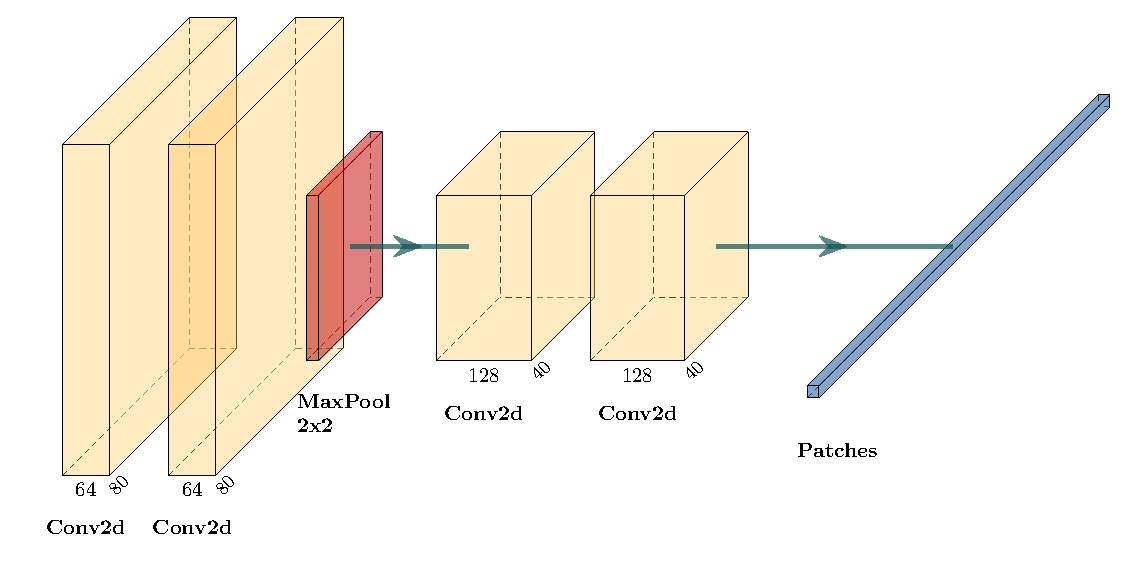
\includegraphics[width=0.9\textwidth]{img/vgg_architecture.pdf}
    \caption{Diagram architektury VGG bloku}
    \label{img:vgg_arch}
\end{figure}
    
    \item \textbf{Poziční kódování} - původní model popsaný v checkpointu obsahoval učící se poziční parametry inicializovaného vektorem s hodnotami 0. Tento přístup byl však neefektivní pro vstupy s různou šířkou. Nyní používáme \textbf{Sinusoidové poziční kódování} \cite{sinusoidal-encoding} pro zachycení prostorových vztahů jak v obrazových datech (2D), tak v sekvencích \LaTeX tokenů (1D). Toto kódování je klíčové pro transformer architekturu, protože umožňuje modelu rozlišovat pozice jednotlivých prvků bez ohledu na jejich vzdálenost. Pro obrazové příznaky se používá 2D varianta, která kombinuje výškovou a šířkovou složku pomocí funkcí sinus a cosinus s různými frekvencemi. Tento přístup vytváří unikátní poziční signál pro každou pozici v mřížce příznaků, přičemž relativní pozice jsou zachyceny pomocí lineárních kombinací těchto trigonometrických funkcí. Pro dekódování \LaTeX sekvence se používá standardní 1D poziční kódování, které následuje stejný princip, ale pouze v jedné dimenzi.
    \item \textbf{Transformer encoder} - zpracovává sekvenci patch embedingů vytvořených z obrázku. V naší implementaci používáme \href{https://docs.pytorch.org/docs/stable/generated/torch.nn.TransformerEncoderLayer.html}{nn.TransformerEncoder z knihovy PyTorch} s několika vrstvami (\textit{num\textunderscore transformer\textunderscore layers=4}), kde každá vrstva obsahuje multi-head self-attention mechanismus (s \textit{nhead=8} hlavami) následovaný feed-forward sítí. Encoder transformuje prostorově uspořádané příznaky z patch embedingu na kontextově bohatou reprezentaci, kde každý vektor obsahuje informace o globálních vztazích v obraze. Tato reprezentace je klíčová pro následné dekódování LaTeX sekvence, protože zachycuje jak lokální detaily matematických symbolů, tak jejich vzájemné prostorové vztahy.
    \item \textbf{Transformer decoder} - převádí zakódované vizuální příznaky na sekvenci LaTeX tokenů. V původní verzi popsané v checkpointu, jsme využívali \textbf{LSTM} s pozorností (attention mechanism) s vrstvou normalizace (LayerNorm). Toto řešení jsme nakonec opustili a jako vhodný dekodér pro transformer kodér jsme zvolili standardní \href{https://docs.pytorch.org/docs/stable/generated/torch.nn.TransformerDecoderLayer.html}{nn.TransformerDecoder} s maskovým self-attention mechanismem, který zajišťuje, že při generování každého tokenu může model vidět pouze předchozí tokeny. Dekodér kombinuje attention na zakódované vizuální příznaky (cross-attention) s maskovaným self-attention na již vygenerované tokeny. Toto umožňuje modelu generovat \LaTeX výstup token po tokenu, přičemž každý nový token je generován s ohledem na vizuální kontext i dosud vygenerovaný text.
\end{itemize}

Model nabízí dva přístupy ke generování výsledné \LaTeX sekvence. Základní \textbf{greedy decoding} vždy vybírá token s nejvyšší pravděpodobností, což je rychlé, ale může vést k suboptimálním výsledkům. Sofistikovanější \textbf{beam search} (výchozí s \textit{beam\textunderscore size=3}) udržuje několik nejpravděpodobnějších sekvencí současně, což poskytuje lepší výsledky za cenu vyšší výpočetní náročnosti.

Každá sekvence začíná speciálním \textbf{<START>} tokenem (1) a končí \textbf{<END>} tokenem (2), čímž model ví, kdy začít a ukončit generování. Pro běžné použití je doporučen beam search, který poskytuje lepší kvalitu rozpoznávání matematických výrazů díky uvažování více možných cest při generování sekvence.

\subsection{Proces trénování}

Trénování začíná inicializací modelu na zvoleném zařízení (CPU/CUDA/MPS) a nastavením optimalizačních komponent. Model využívá \href{https://docs.pytorch.org/docs/stable/generated/torch.optim.AdamW.html}{AdamW} optimizér s váhovým rozpadem pro regularizaci a \href{https://docs.pytorch.org/docs/stable/generated/torch.optim.lr_scheduler.OneCycleLR.html}{OneCycleLR} scheduler pro adaptivní učení. Pro efektivní využití GPU paměti je implementován mixed precision training pomocí automatického přepínání mezi float16 a float32 přesností.

\begin{figure}[h!]
    \centering
    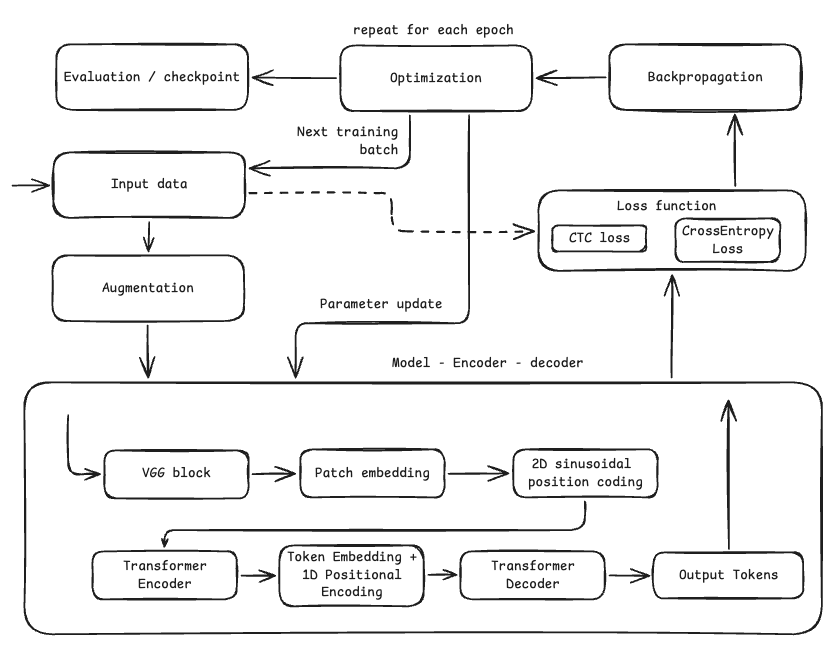
\includegraphics[width=0.9\textwidth]{img/training.png}
    \caption{Trénovací smyčka modelu}
    \label{img:seq_sol}
\end{figure}

\subsubsection{Kombinovaná loss funkce}
Model popsaný v rámci checkpointu používal pouze \textbf{Cross Entropy} loss s label smoothingem (0.15), která optimalizuje přesnost na úrovni jednotlivých tokenů a pomáhá s generalizací. Aktuální model jsme se však pokusili rozšířit o využití sofistikované kombinace dvou loss funkcí, každá s váhou 0.5. \textbf{Connectionist Temporal Classification} (CTC) loss řeší problém zarovnání sekvencí mezi vstupním obrázkem a výstupním LaTeX kódem, umožňující modelu naučit se mapování bez explicitního zarovnání. Tato hybridní loss funkce umožňuje modelu současně se učit globální strukturu matematického výrazu i přesnou tokenizaci.

\subsubsection{Optimalizační strategie}
Trénink využívá gradient accumulation (2 kroky) pro simulaci větších batch size a stabilnější trénink. Learning rate je řízen pomocí OneCycleLR scheduleru, který implementuje warmup fázi (30\% epochy) následovanou cosinovou annealing strategií. Pro prevenci explodujících gradientů je použit gradient clipping s maximální normou 2.0. Mixed precision training s GradScalerem efektivně využívá GPU paměť a zrychluje trénink při zachování numerické stability.


\subsubsection{Monitoring a checkpointing}

Dataset HME obrázků jsme rozdělili na trénovací, validační a testovací sadu v poměru 8:1:1. Na konci každé trénovací epochy jsme použili validační sadu ke zjištění aktuální přesnosti modelu. V průběhu trénování používáme 2 metriky přesnosti.

\begin{enumerate}
    \item \textbf{Token-level accuracy} měří poměr správně predikovaných tokenů na výstupu vůči celkovému počtu tokenů na výstupu. Takto vypočítaná hodnota je sice dobrým přibližným ukazatelem přesnosti modelu, zejména v počátečních fázích trénování, o celkové správnosti výsledku ale příliš dobře nevypovídá, neboť nezahrnuje informaci o celkové struktuře.
    \item \textbf{Sequence accuracy} udává podíl kompletně správně predikovaných sekvencí vůči celkovému počtu sekvencí v sadě -- tato metrika naopak model podhodnocuje, v pozdních fázích trénování se ale může více blížit univerzální metrice \textbf{Expression recognition rate}, která se používá pro porovnání HME recognition modelů.
\end{enumerate}

Proces trénování implementuje mechanismus \textit{early stopping} s trpělivostí 10 epoch pro předcházení přetrénování. Checkpointy jsou ukládány ve třech režimech: při dosažení nejlepší accuracy, při dosažení nejlepší loss a periodicky každých 5 epoch. Toto umožňuje flexibilní obnovu tréninku a výběr optimálního modelu podle různých kritérií.


\subsection{Experimenty}

Vyzkoušeli jsme řadu technik, jak výkon modelu zlepšit, včetně změn architektury, úpravy trénovacího procesu, přidání různých augmentací vstupních trénovacích obrázků. Také jsme rozšířili původní datovou sadu ze soutěže o velké množství obrázků převedených z digitálního formátu InkML. 

\subsubsection{Změny v architektuře modelu}

Původní LSTM architekturu s attention mechanismem jsme nahradili plně transformerovou architekturou. Transformery prokázaly výrazně lepší schopnost paralelizace a efektivnější zpracování dlouhých sekvencí. Zavedení mechanismu multi-head attention (8 hlav) umožnilo modelu paralelně zpracovávat různé aspekty vizuálních rysů rovnic a zlepšilo zachycení dlouhodobých závislostí.

Zásadní změnou bylo nahrazení učitelných pozičních embeddingů sinusoidálním pozičním kódováním. Pro vstupní obraz jsme implementovali 2D sinusoidální pozicování (rozložené na vertikální a horizontální komponenty), zatímco pro dekodér bylo použito standardní 1D sinusoidální kódování. Tato změna vedla ke stabilnějšímu tréninku a lepší schopnosti generalizace.

\subsubsection{Optimalizátor a Scheduler}
\begin{itemize}
    \item AdamW s parametry (lr=3e-4, weight\textunderscore decay=0.01, betas=(0.9, 0.98))
    \item OneCycleLR scheduler s 30\% warmup fází
    \item Gradient accumulation (2 kroky) pro stabilnější trénink
    \item Mixed precision training pro efektivní využití GPU
\end{itemize}

\subsubsection{Implementace kombinované loss funkce}
\begin{itemize}
    \item CTC Loss (váha 0.5) pro sequence alignment
    \item Cross Entropy Loss (váha 0.5) s label smoothing 0.15
    \item Gradient clipping s max\textunderscore norm=2.0
\end{itemize}

\subsubsection{Hyperparametry a další varianty}

\begin{itemize}
    \item \textbf{Počet vrstev TransformerEncoderu}:
    \begin{itemize}
        \item \texttt{layers=2}: nižší kapacita, přesnost stagnovala pod 2\,\%.
        \item \texttt{layers=6}: mírné zlepšení, ale delší trénink bez poklesu validační ztráty.
        \item \texttt{layers=4}: nejlepší kompromis mezi výkonem a paměťovou náročností.
    \end{itemize}
    
    \item \textbf{Dropout}:
    \begin{itemize}
        \item \texttt{dropout=0.0}: výrazné přeučení po cca 10 epochách.
        \item \texttt{dropout=0.3}: stabilnější validační ztráta, ale pomalejší trénink.
        \item \texttt{dropout=0.1}: vyvážené řešení s nejlepším poměrem stability a výkonu.
    \end{itemize}
\end{itemize}

\vspace{1em}

\subsubsection{Analýza výkonnosti}

\begin{itemize}
    \item Trénovací metriky:
    \begin{itemize}
        \item Počáteční loss: $> 5.5$
        \item Konvergovaná loss: $\approx 0.8$
        \item Trénovací přesnost: 98\%
    \end{itemize}
    
    \item Validační metriky:
    \begin{itemize}
        \item Validační loss: $\approx 6.4284$ (bez zlepšení)
        \item Validační přesnost: 3.6\%
    \end{itemize}
    
    \item Testovací metriky:
    \begin{itemize}
        \item Test loss: 6.4398
        \item Testovací přesnost: 3.66\%
    \end{itemize}
\end{itemize}



\subsubsection{Identifikované problémy}

Pozorujeme efekt overfittingu - model vykazuje klasické známky přetrénování, kdy má téměř perfektní výsledky při trénování a už se není schopen zlepšovat, ale validační a testovací metriky na neviděných datech se nezlepšují

Možné příčiny:
\begin{enumerate}
    \item Příliš komplexní model pro danou velikost datasetu
    \item Špatná datová sada obsahující malý počet realistických fotografií ručně napsaných rovnic ze soutěže a data konvertovaná z formátu InkML (digitální formát z tabletu)
    \item Neoptimální hyperparametry, které je pro daný problém nutné jinak nastavit
\end{enumerate}

Tyto výsledky naznačují, že přestože model dokáže efektivně memorovat trénovací data, má významné problémy s generalizací.




\newpage
\section{Závěr}
Tato dokumentace popisuje návrh, implementaci a experimentální vyhodnocení systému KNN-Math pro převod ručně psaných matematických rovnic do formátu \LaTeX. Systém je postaven na moderní architektuře typu encoder–decoder využívající konvoluční síť (VGG blok) pro extrakci vizuálních rysů a transformerový model pro sekvenční generování LaTeX výrazů.

V průběhu vývoje jsme otestovali řadu přístupů ke zlepšení výkonnosti modelu. Zásadní změnou byla náhrada LSTM dekodéru za plně transformerový dekodér a přechod na sinusoidální poziční kódování. Dále jsme zavedli kombinovanou ztrátovou funkci (CTC + Cross Entropy), pokročilé trénovací techniky (gradient accumulation, mixed precision training) a rozšířili datovou sadu o synteticky vygenerované vzorky z formátu InkML.

Ačkoliv model dosahoval vysoké přesnosti na trénovacích datech ($\approx 98\,\%$),  experimenty potvrdily výskyt přeučení -- validační a testovací přesnost se stabilně pohybovala pod 4\%. To naznačuje omezenou schopnost modelu generalizovat na nové vstupy, pravděpodobně kvůli datové nevyváženosti a převažujícímu podílu syntetických vzorků.

Projekt KNN-Math je modulární a otevřený dalšímu rozšiřování. Do budoucna by bylo vhodné zaměřit se na zlepšení kvality a rozmanitosti trénovacích dat, použití větších a realističtějších datasetů, nebo experimentování s jazykovými modely pro zpřesnění dekódované sekvence.
~~


% Citace:
\newpage
\nocite{*}  % Vypsat všechno
\printbibliography[heading=bibintoc, title={Zdroje}]

\end{document} 